\documentclass[aspectratio=169]{beamer}

\setbeamersize{text margin left=5mm, text margin right=5mm}

\defbeamertemplate{headline}{my header}{%
\vskip1pt%
\makebox[0pt][l]{\,\insertshortauthor}%
\hspace*{\fill}\insertshorttitle/\insertshortsubtitle\hspace*{\fill}%
\llap{\insertpagenumber/\insertpresentationendpage\,}
}
\setbeamertemplate{headline}[my header]

\let\olditem\item
\renewcommand{\item}{\setlength{\itemsep}{\fill}\olditem}

\usepackage{bm}
\usepackage{graphicx}
\usepackage{caption}
\usepackage{soul}
\usepackage{tkz-euclide}
\usetikzlibrary{calc}
\usepackage[]{algorithm2e}
\usepackage{changepage}
\usepackage{amssymb}
\usepackage{xcolor}
\usepackage{mathtools}
\usepackage{tcolorbox}
\usepackage{tikz}
\usepackage{tikz-3dplot}
\usepackage{tkz-euclide}
\usepackage{pgfplots}
\pgfplotsset{width=5cm,compat=1.3}
\usepackage{circuitikz}
\usepackage{mleftright}
% \usepackage{algorithm,algorithmic}
\usetikzlibrary{arrows.meta, decorations.pathreplacing, positioning, shapes.geometric}
\usetikzlibrary{arrows}

\usepackage{pgfplots}
\usetikzlibrary{plotmarks}
\pgfplotsset{width=7cm,compat=1.8}
\pgfplotsset{compat=1.17}

\usetikzlibrary{positioning}
% \usepackage[math]{cellspace}
% \cellspacetoplimit 4pt
% \cellspacebottomlimit 4pt
%\usetikzlibrary{arrows.meta}
% sqare of half axes
\newcommand{\asa}{3}
\newcommand{\bsa}{1}
\newcommand{\csa}{0.25}
% view angle
\tdplotsetmaincoords{70}{135}


%% Fonts
\usefonttheme{professionalfonts}
\usefonttheme{serif}

\DeclareCaptionLabelFormat{blank}{}
\captionsetup[figure]{labelformat=blank}

%% Math definitions
\def\mf{\ensuremath\mathbf}
\def\mb{\ensuremath\mathbb}
\def\mc{\ensuremath\mathcal}
\def\lp{\ensuremath\left(}
\def\rp{\ensuremath\right)}
\def\lv{\ensuremath\left\lvert}
\def\rv{\ensuremath\right\rvert}
\def\lV{\ensuremath\left\lVert}
\def\rV{\ensuremath\right\rVert}
\def\lc{\ensuremath\left\{}
\def\rc{\ensuremath\right\}}
\def\ls{\ensuremath\left[}
\def\rs{\ensuremath\right]}
\def\bmx{\ensuremath\begin{bmatrix*}[r]}
\def\emx{\ensuremath\end{bmatrix*}}
\def\bmxc{\ensuremath\begin{bmatrix*}[c]}
\def\R{\ensuremath\mb{R}}
\def\t{\lp t\rp}
\def\k{\ls k\rs}

\newcommand{\demoex}[2]{\onslide<#1->\begin{color}{black!60} #2 \end{color}}
\newcommand{\demoexc}[3]{\onslide<#1->\begin{color}{#2} #3 \end{color}}
\newcommand{\anim}[3]{\onslide<#1->{\begin{color}{#2!60} #3 \end{color}}}
\newcommand{\ct}[1]{\lp #1\rp}
\newcommand{\dt}[1]{\ls #1\rs}
\newcommand{\cols}[2]{\begin{columns}[#1] #2 \end{columns}}
\newcommand{\col}[2]{\begin{column}{#1} #2 \end{column}}

%% Mycolors
\definecolor{myred}{RGB}{192,0,0}
\definecolor{mygray}{RGB}{100,100,100}

%% Custom beamer color
\setbeamercolor{title}{fg=myred}
\setbeamercolor{subtitle}{fg=myred}
\setbeamerfont{title}{series=\bfseries}
% \setbeamercolor{frametitle}{bg=myred, fg=white}
\setbeamercolor{frametitle}{bg=mygray!10!, fg=myred}
\setbeamerfont{frametitle}{series=\bfseries}
\setbeamercolor{item}{fg=mygray}
\setbeamercolor{title in head/foot}{fg=myred}

% Move header to footer
\setbeamertemplate{headline}{}
\setbeamertemplate{footline}{
  \begin{beamercolorbox}[wd=\paperwidth,ht=2.25ex,dp=1ex,center]{footline}
    \inserttitle\hfill\insertauthor\hfill\insertdate\hfill\insertframenumber{}
  \end{beamercolorbox}
}

\pgfplotsset{
colormap={whitered}{color(0cm)=(white); color(1cm)=(orange!75!red)}
}


\title{Applied Linear Algebra in Data Analysis}

% A subtitle is optional and this may be deleted
\subtitle{Introduction to Constrained Optimization}

\author{Sivakumar Balasubramanian}
% - Give the names in the same order as the appear in the paper.
% - Use the \inst{?} command only if the authors have different
%   affiliation.

\institute[Christian Medical College] % (optional, but mostly needed)
{
  \inst{}%
  Department of Bioengineering\\
  Christian Medical College, Bagayam\\
  Vellore 632002
}
% - Use the \inst command only if there are several affiliations.
% - Keep it simple, no one is interested in your street address.

\date{}
% - Either use conference name or its abbreviation.
% - Not really informative to the audience, more for people (including
%   yourself) who are reading the slides online

\subject{Lecture notes on ALADA}
% This is only inserted into the PDF information catalog. Can be left
% out. 

% If you have a file called "university-logo-filename.xxx", where xxx
% is a graphic format that can be processed by latex or pdflatex,
% resp., then you can add a logo as follows:

% \pgfdeclareimage[height=0.5cm]{university-logo}{university-logo-filename}
% \logo{\pgfuseimage{university-logo}}

% Delete this, if you do not want the table of contents to pop up at
% the beginning of each subsection:
\AtBeginSubsection[]
{
  \begin{frame}<beamer>{Outline}
    \tableofcontents[currentsection,currentsubsection]
  \end{frame}
}

% Let's get started
\begin{document}

\pgfplotsset{
  compat=1.8,
  colormap={whitered}{color(0cm)=(white); color(1cm)=(orange!75!red)}
}


\begin{frame}
  \titlepage
\end{frame}


\begin{frame}[t]{Overdetermined System of linear equations}
\begin{itemize}
\item For a tall, skinny matrix $\mathbf{A} \in \mathbb{R}^{m \times n}$, there is a solution to $\mathbf{Ax} = \mathbf{b}$, only when $\mathbf{b} \in C\left(\mathbf{A}\right)$.

\[ \mathbf{b} = \sum_{i=1}^{n} \mathbf{v}_i a_i = \mathbf{V}\mathbf{a}; \,\,\, \mathbf{a} \in \mathbb{R}^n, \,\,\, \mathbf{V} = \begin{bmatrix*}\mathbf{v}_1 & \mathbf{v}_2 & \cdots & \mathbf{v}_n\end{bmatrix*} \in \mathbb{R}^{n \times n} \]

\item Can we have an approximate solution when $\nexists \mathbf{x}$ such that $\mathbf{Ax} = \mathbf{b}$?

Let us define ``approximate'' solution $\hat{\mathbf{x}}$ as the one that minimizes $\left\lVert \mathbf{b} - \mathbf{A}\hat{\mathbf{x}}\right\rVert_2^2, \,\,\,\, \forall \mathbf{x} \in \mathbb{R}^n$ . This is the \textit{least squares problem}.

\[ \text{Given } \mathbf{A} \text{ and } \mathbf{b}, \text{ choose } \hat{\mathbf{x}} \text{ such that} \] \[ \text{minimize }\,\,\, \left\lVert \mathbf{b} - \mathbf{Ax}\right\rVert_2^2 \]

\item $\mathbf{A}$ and $\mathbf{b}$ come from the data.

\item $\left\lVert \mathbf{b} - \mathbf{Ax}\right\rVert^2$ is called the objective function.
\end{itemize}
\end{frame}

\begin{frame}[t]{Least Squares Problem}
\vspace{-0.25cm}
\begin{small}
\[ 
    \begin{rcases*}
        2x & = 1 \\
        -1x & = -2 \\
        \sqrt{2}x & = 0
    \end{rcases*} \, \longrightarrow \mathbf{Ax} = \mathbf{b}, \,\,\, \mathbf{A} = \begin{bmatrix*}[r] 2\\-1\\\sqrt{2}\end{bmatrix*}, \,\, \mathbf{x} \in \mathbb{R}, \,\, \mathbf{b} \in \begin{bmatrix*}[r]1\\-2\\0\end{bmatrix*}
\]

\[
    \left\lVert \mathbf{b} - \mathbf{Ax}\right\rVert^2 = \left(1 - 2x\right)^2 + \left(-2 + x\right)^2 + \left(\sqrt{2}x\right)^2 = 7x^2 - 8x + 5 \geq 0
\]
\end{small}

\vspace{-0.25cm}

\begin{columns}
\begin{column}{0.5\textwidth}
\begin{center}
    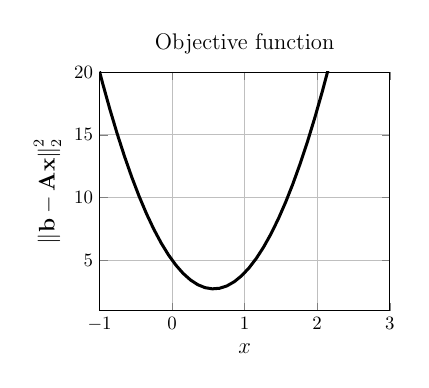
\begin{tikzpicture}[scale=0.68]
        \begin{axis}[xmin=-1,xmax=3,ymax=20,samples=100,grid=major,xlabel={{\large $x$}},ylabel={{\large $\left \lVert \mathbf{b} - \mathbf{Ax}\right\rVert_2^2$}},title={{\large Objective function}}]
        \addplot[black, ultra thick](x, 7*x*x - 8*x + 5);
    \end{axis}
    \end{tikzpicture}
\end{center}
\end{column}

\begin{column}{0.5\textwidth}
The objective function assumes its minimum value, at $\hat{\mathbf{x}} = \frac{4}{7}$ 
\end{column}
\end{columns}
\end{frame}


\begin{frame}[t]{Least Squares Problem}
\vspace{-0.25cm}
\begin{small}
\[ 
    \begin{rcases*}
    2x_1 - x_2 & = 2 \\
    -x_1 + x_2 & = 1 \\
    3x_1 + 2x_2 & = -1
    \end{rcases*} \, \longrightarrow \mathbf{Ax} = \mathbf{b}, \,\,\, \mathbf{A} = \begin{bmatrix*}[r] 2 & -1\\ -1 & 1\\3 & 2\end{bmatrix*}, \,\, \mathbf{x} = \begin{bmatrix*}[r] x_1\\ x_2\end{bmatrix*} , \,\, \mathbf{b} \in \begin{bmatrix*}[r]2\\1\\-1\end{bmatrix*}
\]

\[
    \left\lVert \mathbf{b} - \mathbf{Ax}\right\rVert^2 = 14x_1^2 + 6x_2^2 + 6x_2 + 6x_1x_2 + 6 \geq 0
\]
\end{small}

\vspace{-0.25cm}

\begin{columns}
\begin{column}{0.6\textwidth}
\begin{center}
    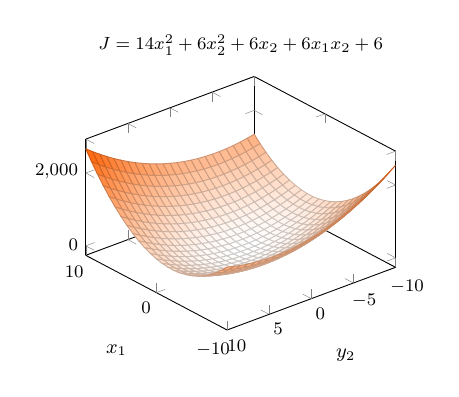
\begin{tikzpicture}[scale=0.8]
    \begin{axis}[
        title={\footnotesize{$J = 14x_1^2+6x_2^2+6x_2+6x_1x_2+6$}}, 
        xlabel=$x_1$, ylabel=$y_2$,
        view={230}{40},small,
    ]
    \addplot3[
        surf,
        domain=-10:10,
        domain y=-10:10,
    ] {(14*x*x)+(6*y*y)+(6*y)+(6*x*y)+6};
    \end{axis}
    \end{tikzpicture}
\end{center}
\end{column}

\begin{column}{0.4\textwidth}
The objective function assumes it minimum value at, $\hat{x}_1 = \frac{52}{75}$ and $\hat{x}_2 = \frac{3}{25}$.
\end{column}
\end{columns}
\end{frame}


\begin{frame}[t]{Least Squares Methods}
\begin{itemize}
    \item The general solution to this least squares problem can be derived using calculus. Let $f\left(\mathbf{x}\right) = \left\lVert \mathbf{b} - \mathbf{Ax} \right\rVert$
    \[ \nabla f\left(\mathbf{x}\right) = 0 \longrightarrow 
    \begin{bmatrix*}
    \frac{\partial f}{\partial x_1}\\
    \vdots \\
    \frac{\partial f}{\partial x_n}\\
    \end{bmatrix*} = 0
    \]

    Going through the algebra, we end up with the following expression for $\hat{\mathbf{x}}$ that minimizes $f\left(\mathbf{x}\right)$,
    \[  \underbrace{\mathbf{A}^T\mathbf{A}\hat{\mathbf{x}} = \mathbf{A}^T\mathbf{b}}_\text{Normal Equations} \]
    $\mathbf{A}$ is full rank, $\implies$ $\mathbf{A}^T\mathbf{A}$ is invertible.
    \[ \implies \hat{\mathbf{x}} = \underbrace{\left(\mathbf{A}^T\mathbf{A}\right)^{-1}\mathbf{A}^T}_\text{Pseudo-inverse}\mathbf{b} = \mathbf{A}^{\dagger}\mathbf{b} \]
\end{itemize}
\end{frame}


\begin{frame}[t]{Least Squares Methods}
\begin{footnotesize}
\begin{itemize}
    \item $\hat{\mathbf{x}}$ is the approximate least squares solution. $\hat{\mathbf{b}} = \mathbf{A}\hat{\mathbf{x}}$, which is in general not equal to $\mathbf{b}$. \textit{When is $\mathbf{b} = \hat{\mathbf{b}}$?}
    \item We know two things about $\hat{\mathbf{b}}$,
    \begin{enumerate}
        \item $\hat{\mathbf{b}} \in C\left(\mathbf{A}\right)$: $\hat{\mathbf{b}}$ is the column space of $\mathbf{A}$.
        \item $\left\lVert \mathbf{b} - \hat{\mathbf{b}}\right\rVert$ is minimum.
    \end{enumerate}
\end{itemize}
\end{footnotesize}

% \vspace{0.5cm}

\begin{columns}
\begin{column}{0.5\textwidth}
    \tdplotsetmaincoords{65}{55} 
    \begin{tikzpicture}[scale=1.5, tdplot_main_coords, axis/.style={-stealth,gray,thin}, vector/.style={-stealth, black, thick}, vector hat/.style={-stealth,gray,thick}, vector proj/.style={-stealth,violet,ultra thin}]

    %standard tikz coordinate definition using x, y, z coords
    \coordinate (O) at (0,0,0);

    \fill[gray!50,opacity=0.6] (-1,-1,0) -- (2,-1,0) -- (2,2,0) -- (-1,2,0) -- (-1,-1,0);

    %draw axes
    \draw[axis] (0,0,0) -- (1.3,-0.2,0) node[right]{$\mathbf{a}_1$};
    \draw[axis] (0,0,0) -- (0.4,0.8,0) node[right]{$\mathbf{a}_2$};

    %draw a vector from O to P
    \draw[vector] (0,0,0) -- (1,1,0.7) node[above]{$\mathbf{b}$};
    \draw[vector hat] (0,0,0) -- (1,1,0) node[right]{$\hat{\mathbf{b}}=\mathbf{A}\hat{\mathbf{x}}$};
    \draw[vector proj] (1,1,0) -- (1,1,0.7) node[xshift=0.7cm,yshift=-0.6cm]{$\mathbf{b} - \mathbf{A}\hat{\mathbf{x}}$};

    \node[gray,left] at (0,0,0) {$\mathbf{0}$};
    \node[gray] at (-0.5,-0.5,0) {$C\left(\mathbf{A}\right)$}; 
    \end{tikzpicture}
\end{column}
\begin{column}{0.55\textwidth}
\begin{footnotesize}
$\left \lVert \mathbf{b} - \mathbf{A}\hat{\mathbf{x}}\right\rVert_2^2$ is minimum $\implies \left(\mathbf{b} - \mathbf{A}\hat{\mathbf{x}}\right) \perp \mathbf{A}\hat{\mathbf{x}}$
\[ \left(\mathbf{A}\hat{\mathbf{x}}\right)^T\left(\mathbf{b} - \mathbf{A}\hat{\mathbf{x}}\right) = 0 \implies \hat{\mathbf{x}}^T\underbrace{\left(\mathbf{A}^T\mathbf{b} - \mathbf{A}^T\mathbf{A}\hat{\mathbf{x}}\right)}_\text{Normal Equations} = 0\]

\textit{The least squares approximate solution of $\mathbf{Ax} = \mathbf{b}$ is the solution solution to the equation $\mathbf{Ax} = \hat{\mathbf{b}}$, where $\hat{\mathbf{b}}$ is the projection of $\mathbf{b}$ onto the column space of $\mathbf{A}$ $\left(C\left(\mathbf{A}\right)\right)$.}
\end{footnotesize}
\end{column}
\end{columns}
\end{frame}


\begin{frame}[t]{Multi-Objective Least Squares}
\begin{small}
\begin{itemize}
    \item There are applications where there is more than one objective that must be optimized,
    \[ J_1 = \left\lVert \mathbf{A}_1\mathbf{x} - \mathbf{b}_1 \right\rVert^2, \,\,
    J_2 = \left\lVert \mathbf{A}_2\mathbf{x} - \mathbf{b}_2 \right\rVert^2, \,\,
    \ldots \,\,
    J_k = \left\lVert \mathbf{A}_k\mathbf{x} - \mathbf{b}_k \right\rVert^2, \,\,
    \]
    and often these are conflicting objectives.

    \item We can define a single objective function $J$ that is takes into account the different objective functions.
    \[ J = \sum_{i=1}^k\rho_iJ_i, \,\,\, \rho_i > 0, \,\,\,\, \forall 1 \leq i \leq k\]

    \item The $\rho_i$s indicate the relative weightage given to the individual objectives.
    \[ J = J_1 + \sum_{i=2}^k\rho_iJ_i \]
\end{itemize}
\end{small}
\end{frame}


\begin{frame}[t]{Multi-Objective Least Squares}
\begin{small}
    \[ \begin{split}
    J & = \rho_1\left\lVert \mathbf{A}_1\mathbf{x} - \mathbf{b}_1 \right\rVert^2 + \ldots + \rho_k\left\lVert \mathbf{A}_k\mathbf{x} - \mathbf{b}_k \right\rVert^2 \\
     & = \left\lVert \sqrt{\rho_1}\mathbf{A}_1\mathbf{x} - \sqrt{\rho_1}\mathbf{b}_1 \right\rVert^2 + \ldots + \left\lVert \sqrt{\rho_k}\mathbf{A}_k\mathbf{x} - \sqrt{\rho_k}\mathbf{b}_k \right\rVert^2
    \end{split}
    \]
    \[ J = \left\lVert 
    \begin{bmatrix*}\sqrt{\rho_1}\mathbf{A}_1\\\sqrt{\rho_2}\mathbf{A}_2\\\vdots\\\sqrt{\rho_k}\mathbf{A}_k\\\end{bmatrix*}\mathbf{x} - \begin{bmatrix*}\sqrt{\rho_1}\mathbf{b}_1\\\sqrt{\rho_2}\mathbf{b}_1\\\vdots\\\sqrt{\rho_k}\mathbf{b}_k\\\end{bmatrix*}\right\rVert^2
    = \left\lVert \mathbf{\tilde{A}}\mathbf{x} - \mathbf{\tilde{b}}\right\rVert^2
    \implies \hat{x} = \left(\mathbf{\tilde{A}}^T\mathbf{\tilde{A}}\right)^{-1}\mathbf{\tilde{A}}^T\mathbf{\tilde{b}}
    \]

    The columns of $\mathbf{\tilde{A}}$ are must be independent, which happens if the columns of at least one of the $\mathbf{A}_i$s is independent.

    Consider a two objective case, $J = J_1 + \rho J_2$.
    \[ \hat{\mathbf{x}} = \begin{cases}
    \mathrm{argmin}_x \left\lVert \mathbf{A}_1\mathbf{x} - \mathbf{b}_1\right\rVert^2 & \rho = 0\\
    \mathrm{argmin}_x \left\lVert \mathbf{A}_2\mathbf{x} - \mathbf{b}_2\right\rVert^2 & \rho \rightarrow \infty 
    \end{cases}
    \]
    \end{small}
\end{frame}


\begin{frame}[t]{Multi-Objective Least Squares}
    Consider a problem with the objecrive function, $J\ct{\mf{x}} = J_1\ct{\mf{x}} + \rho J_2\ct{\mf{x}}$, where $\mf{x} = \mb{R}^3$.

    \begin{figure}
        \centering
        \includegraphics[width=.7\textwidth]{../../analysis/leastsquares/output/multiobj_soln.png}
    \end{figure}
\end{frame}


\begin{frame}[t]{Multi-Objective Least Squares}
    \begin{columns}
        \begin{column}{0.3\textwidth}
        {\small Any solution that lies on this curve is called the \textit{Pareto optimal} solution. There exists no solution $\tilde{\mathbf{x}}$, such that $J_1\left(\tilde{\mathbf{x}}\right) \leq J_1\left(\hat{\mathbf{x}}\right) \,\,\, \text{and} \,\,\, J_2\left(\tilde{\mathbf{x}}\right) \leq J_2\left(\hat{\mathbf{x}}\right)$ where, both inqualities hold strictly.}
        \end{column}
        
        \begin{column}{0.65\textwidth}
        \begin{figure}
            \centering
            \includegraphics[width=0.8\textwidth]{../../analysis/leastsquares/output/multiobj_opt.png}
        \end{figure}
    \end{column}
    \end{columns}
\end{frame}


\begin{frame}[t]{Multi-Objective Least Squares}
\begin{small}
\begin{itemize}
    \item Multi-objective least squares methods play an important role in both control and estimation problems.
    
    \item Appropriate choice of the objective functions can also help deal with conditions where the columns of $A_i$ are not independent. Consider the following example,
    \[ J_1 = \left\lVert \mathbf{A}_1\mathbf{x} - \mathbf{b}_1 \right\rVert^2 \,\,\, \text{ and } \,\,\, J_2 = \left\lVert \mathbf{A}_2\mathbf{x} - \mathbf{b}_2\right\rVert^2 \]
    where, $\mathbf{A}_1 \in \mathbb{R}^{m_1 \times n}$ and $\mathbf{A}_2 \in \mathbb{R}^{m_2 \times n}$, such that $m_1, m_2 < n$. Thus, the columns of $A_1$ and $A_2$ are not independent!
    However, if $m_1 + m_2 \geq n$, then it is possible that the columns of $\tilde{A}$ are independent.

    \item This is called \textbf{regularized least squares}.

    \item \textbf{Tichonov regularization}: $J = \left\lVert \mathbf{Ax} - \mathbf{y}\right\rVert^2 + \rho \left\lVert \mathbf{x} \right\rVert^2$, where $\rho > 0$.
    \[ \mathbf{\tilde{A}} = \begin{bmatrix*}\mathbf{A}\\\sqrt{\rho}\mathbf{I}\end{bmatrix*} \implies \hat{\mathbf{x}} =  \left(\mathbf{A}^T\mathbf{A} + \rho \mathbf{I}\right)^{-1}\mathbf{A}^T\mathbf{b} \]
\end{itemize}
\end{small}
\end{frame}


\begin{frame}[t]{Multi-Objective Least Squares}
\begin{small}
\begin{itemize}
    \item \textbf{Tichonov regularization}: $J = \left\lVert \mathbf{Ax} - \mathbf{y}\right\rVert^2 + \rho \left\lVert \mathbf{x} \right\rVert^2$, where $\rho > 0$.
    \[ \tilde{\mathbf{A}} = \begin{bmatrix*}\mathbf{A}\\\sqrt{\rho}\mathbf{I}\end{bmatrix*} \implies \hat{\mathbf{x}} =  \left(\mathbf{A}^T\mathbf{A} + \rho \mathbf{I}\right)^{-1}\mathbf{A}^T\mathbf{b} \]
    \item $\hat{\mathbf{x}}$ gives a unique solution in minimizing $J$, even when $\mathbf{A}$ is not full rank.
    \item Even when $\mathbf{A}$ is full rank, the regularization term can be used to improve the condition number of the matrix.
\end{itemize}
\end{small}
\end{frame}


\begin{frame}[t]{Constrained Least Squares}
\begin{small}
\begin{itemize}
    \item \textbf{Problem}:
    \vspace{-0.5cm}
    \[
    \begin{split}
    \text{minimize} & \,\,\, \left\lVert \mathbf{Ax} - \mathbf{b}\right\rVert^2\\
    \text{subject to} & \,\,\, \mathbf{Cx} = \mathbf{d}
    \end{split} 
    \]
    where, $\mathbf{A} \in \mathbb{R}^{m \times n}$, $\mathbf{x} \in \mathbb{R}^n$, $\mathbf{b} \in \mathbb{R}^m$, $\mathbf{C} \in \mathbb{R}^{p \times n}$ and $\mathbf{d} \in \mathbb{R}^p$.

    \item This can be solved using the \textit{method of Lagrange multipliers}. When we do this, we finally arrive the following set of equations, called the \textit{Karush-Kuhn-Tucker} (KKT) equation,
    \[  2\left(\mathbf{A}^T\mathbf{A}\right)\hat{\mathbf{x}} - 2\mathbf{A}^T\mathbf{b} + \mathbf{C}^T\hat{z} = 0  \]
    \[  \begin{bmatrix*}
    2\left(\mathbf{A}^T\mathbf{A}\right) & \mathbf{C}^T\\
    \mathbf{C} & 0\\ 
    \end{bmatrix*}\begin{bmatrix*} \hat{\mathbf{x}}\\ \hat{\mathbf{z}}\end{bmatrix*} = \begin{bmatrix*} 2\mathbf{A}^T\mathbf{b} \\ \mathbf{d}\end{bmatrix*} \]
    \item The coefficient matrix on the LHS of the KKT equation a square matrix of dimensions $\left(n+p\right) \times \left(n+p\right)$ is invertible, if and only if, $\begin{bmatrix}\mathbf{A}\\\mathbf{C}\end{bmatrix}$ is full rank.
\end{itemize}
\end{small}
\end{frame}

\end{document}